\appendix

\section{Proof of No $PID_{RP}$ Collision}
\label{proof-rp-collision}
Given $PID_{RP} = [t]ID_{RP}$, the probability that $PID_{RP}$ designates another RP with $ID_{RP'}$ is \emph{negligible}, %This means that $PID_{RP}$ cannot be associated with any other RPs in the system.
so $PID_{RP}$ designates only the target RP with $ID_{RP}$ in the system.
Finding $t$ and $t'$ that satisfy $[t]ID_{RP_j} = [t']ID_{RP_{j'}}$, can be described as a $PID_{RP}$-collision game $\mathcal{G}_c$ between an adversary and a challenger: the adversary receives from the challenger a finite set of RP identities, i.e., $ID_{RP_1}$, ..., $ID_{RP_m}$, where $m$ is the  finite number of RPs in the system, and outputs $(a, b, t, t')$ where $a \neq b$. If $[t]ID_{RP_a}=[t']ID_{RP_b}$, which occurs with a probability ${\rm Pr}_s$, the adversary succeeds in this game.
%The attack success probability is defined as ${\rm Pr}_s$.

As depicted in Figure \ref{fig:ecdlp_algorithm}, we then design a probabilistic polynomial time (PPT) algorithm $\mathcal{D}^*_c$ based on $\mathcal{G}_c$, to solve the ECDLP: find a number $x \in \mathbb{Z}_n$ satisfying $Q = [x]G$, where $Q$ is a point on $\mathbb{E}$ and $G$ is a generator on $\mathbb{E}$ of order $n$.

%where ${\rm Pr}\{\}$ denotes the probability.
%where $k$ denotes the security parameter and $\epsilon_{c}(k)$ becomes negligible when $k$ is sufficiently large.
%For any sufficiently large $k$, $m \ll 2^k$ since $m$ is a finite integer.

\begin{figure}[hbt]
  \centering
  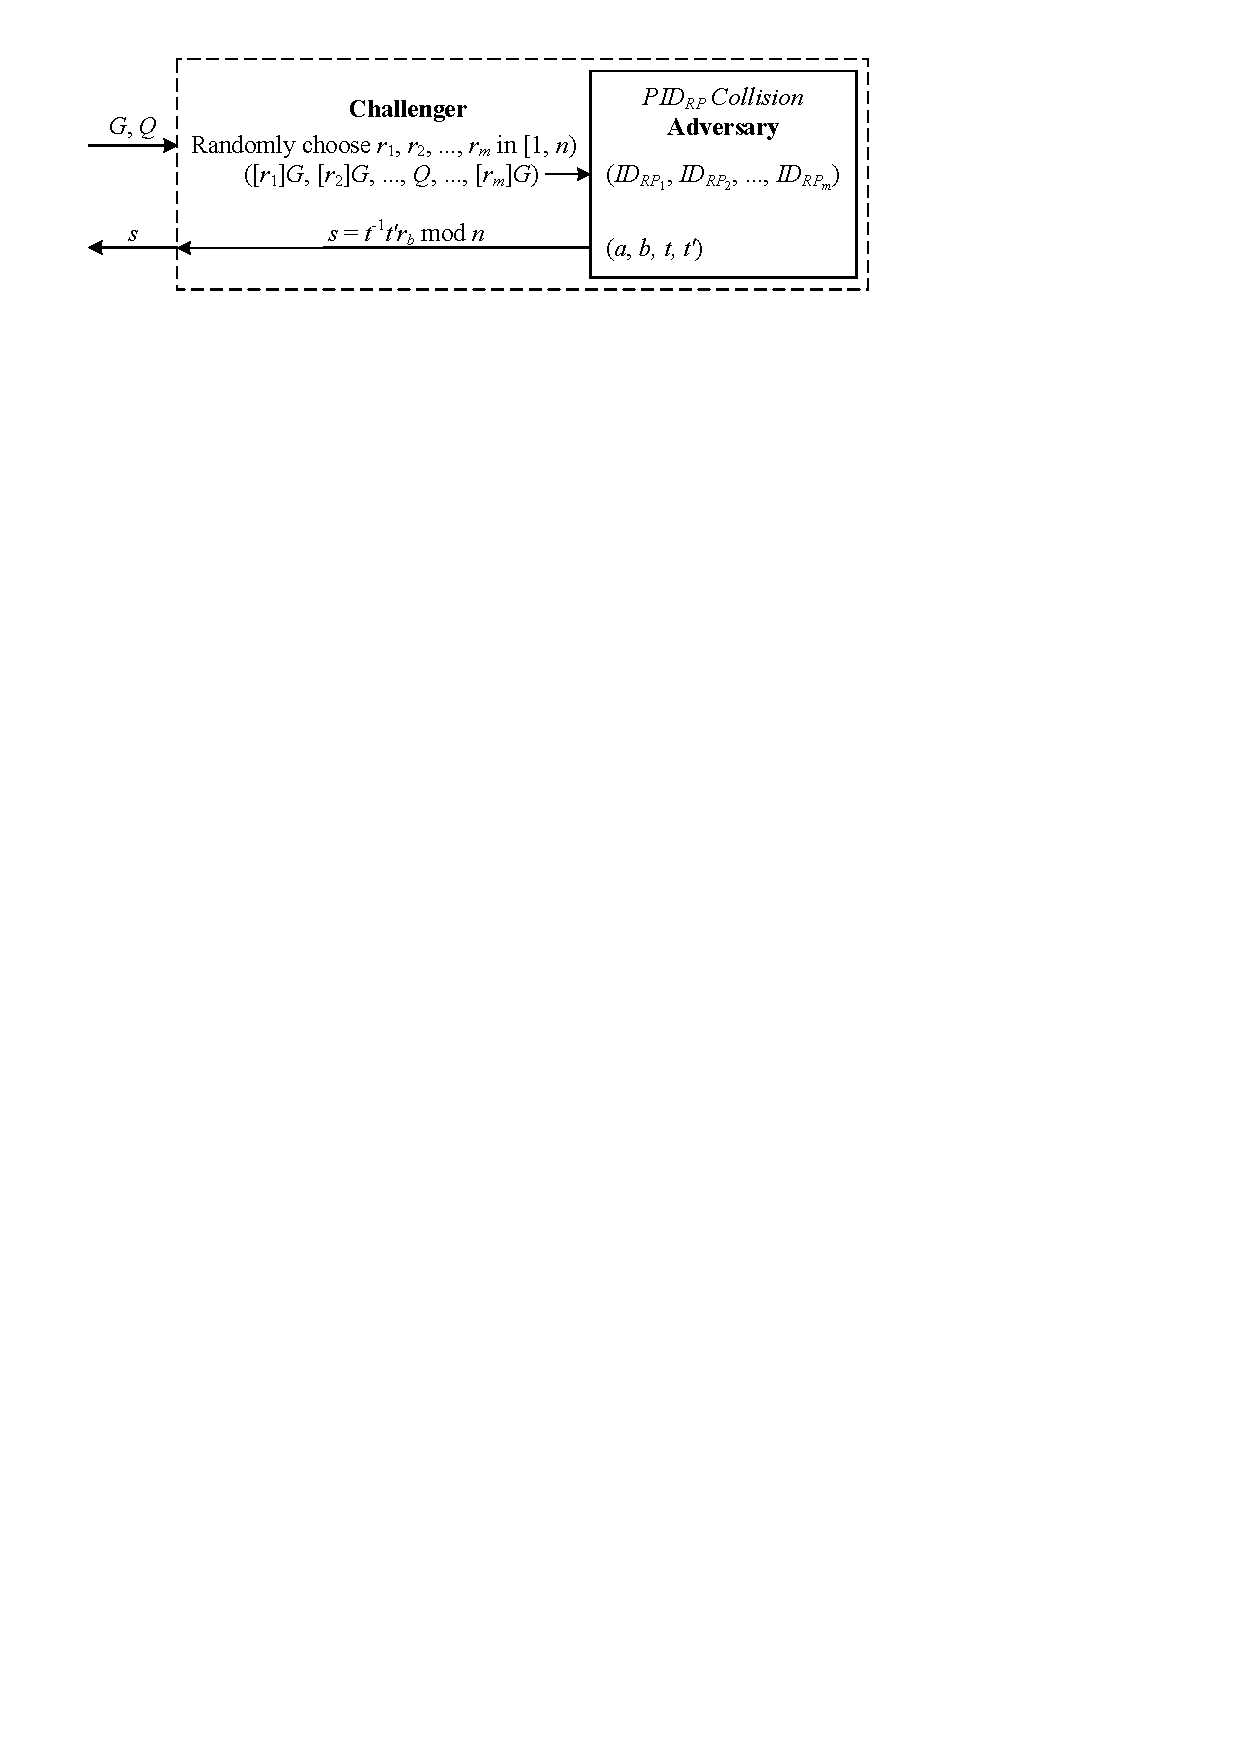
\includegraphics[width=0.96\linewidth]{fig/ecdlp_algorithm.pdf}
  \caption{The PPT algorithm $\mathcal{D}^*_c$ constructed based on the $PID_{RP}$ collision game to solve the ECDLP.}
  \label{fig:ecdlp_algorithm}
\end{figure}

The algorithm $\mathcal{D}^*_c$ works as below.
The input of $\mathcal{D}^*_c$ is in the form of ($G, Q$). On receiving an input ($G$, $Q$), the challenger first randomly chooses $r_1, \cdots, r_m$ in $\mathbb{Z}_n$ to calculate $[r_1]G, \cdots, [r_m]G$.
Then, it randomly chooses $j \in [1,m]$, replaces $[r_j]G$ with $Q$, and sends $m$ RP identities to the adversary, which returns the result ($a$, $b$, $t$, $t'$). Finally, the challenger calculates $s = t^{-1}t'r_b \bmod n$ and returns $s$ as the output of $\mathcal{D}^*_c$.

If the adversary succeeds in $\mathcal{G}_c$ and $[r_a]G$ happens to be replaced with $Q$, then $\mathcal{D}^*_c$ outputs $s=t^{-1}t'r_b =x$ because $[tr_a]G = [t]Q = [t'r_b]G$. For the adversary, $Q$ is indistinguishable from any other RP identities in the input set, as $[r_j]G$ is randomly replaced by the challenger.
Hence, the probability of solving the ECDLP using $\mathcal{D}^*_c$ is formulated as:
\begin{equation*}
{\rm Pr}\{\mathcal{D}^*_c(G, [x]G)=x\} = {\rm Pr}\{s = x\}={\rm Pr}\{a=j\}{\rm Pr}_s=\frac{1}{m}{\rm Pr}_s
\end{equation*}

If the probability of finding $t$ and $t'$ satisfying $[t]ID_{RP_j} = [t']ID_{RP_{j'}}$ is non-negligible, the adversary would have advantages  in $\mathcal{G}_c$ and ${\rm Pr}_s$ is non-negligible regardless of the security parameter $\lambda$.
Thus, we would find that ${\rm Pr}\{\mathcal{D}^*_c(G, [x]G)=x\}$ also becomes non-negligible even when $\lambda$ is sufficiently large, because $m$ is a finite integer and $m \ll 2^\lambda$.
This violates the ECDLP assumption. Therefore, the probability of finding $t$ and $t'$ that satisfy $[t]ID_{RP_j} = [t']ID_{RP_{j'}}$ is negligible.
